\subsection{Anatomical Prior-aware Feature Enhancement}
\label{subsec:apfe}

Existing temporal models \cite{deng2024memsam,mm25_echovim,ICCV25_gdkvm} mainly rely on discrete memory or linear aggregation, treating ultrasound speckle and anatomical boundaries without distinction.
This approach lacks physical priors, leading to representation drift under rapid cardiac deformations and severe noise.
To address this issue, we propose the \emph{Anatomical Prior-aware Feature Enhancement} module (\cref{fig:apfe}).
Unlike standard visual encoders, APFE explicitly accounts for depth-dependent acoustic attenuation by decomposing the feature space into local acoustic fields and structural residuals, decoupling anatomical boundaries from stochastic noise and providing a stable basis for long-term propagation.

\noindent
\textbf{Intensity decoupling via local acoustic fields.}
Echocardiographic signals are corrupted by both stochastic speckle and severe depth-dependent acoustic attenuation \cite{8265568,WANG201925}.
The attenuation follows an approximately exponential decay with depth, which induces a spatially-varying acoustic bias field that confounds genuine tissue contrast.
Relying on a global threshold fails to account for this spatial heterogeneity.
Instead, we formalize the acoustic prior by decomposing the intermediate feature map $\mathbf{X}_t \in \mathbb{R}^{B\times C\times H\times W}$ into a low-frequency ambient acoustic field and high-frequency structural residuals.
Specifically, we estimate the spatially-varying acoustic bias field $\mathbf{M}_t \in \mathbb{R}^{B\times C\times H\times W}$ via large-kernel average pooling:
\begin{equation}
    \mathbf{M}_t = \mathrm{AvgPool}_{K \times K}(\mathbf{X}_t),
\end{equation}
where $K$ defines the receptive field of the acoustic environment.
By treating $\mathbf{M}_t$ as a local physical estimator of the acoustic bias field, we derive the polarity-aware components:
\begin{equation}
    \mathbf{X}_t^{+} = \mathrm{ReLU}(\mathbf{X}_t - \mathbf{M}_t), \quad \mathbf{X}_t^{-} = \mathrm{ReLU}(\mathbf{M}_t - \mathbf{X}_t).
\end{equation}
This dual-ReLU decomposition implicitly performs background-foreground decoupling: $\mathbf{X}_t^{+}$ isolates high-frequency structural edges (\eg, myocardium boundaries) by retaining only positive residuals above the local bias, while $\mathbf{X}_t^{-}$ captures low-response homogeneous regions (\eg, blood pools).
This formulation yields a lossless residual decomposition ($\mathbf{X}_t = \mathbf{X}_t^{+} - \mathbf{X}_t^{-} + \mathbf{M}_t$) that preserves all high-frequency details while filtering out low-frequency intensity fluctuations.

\begin{figure}[t]
    \centering
        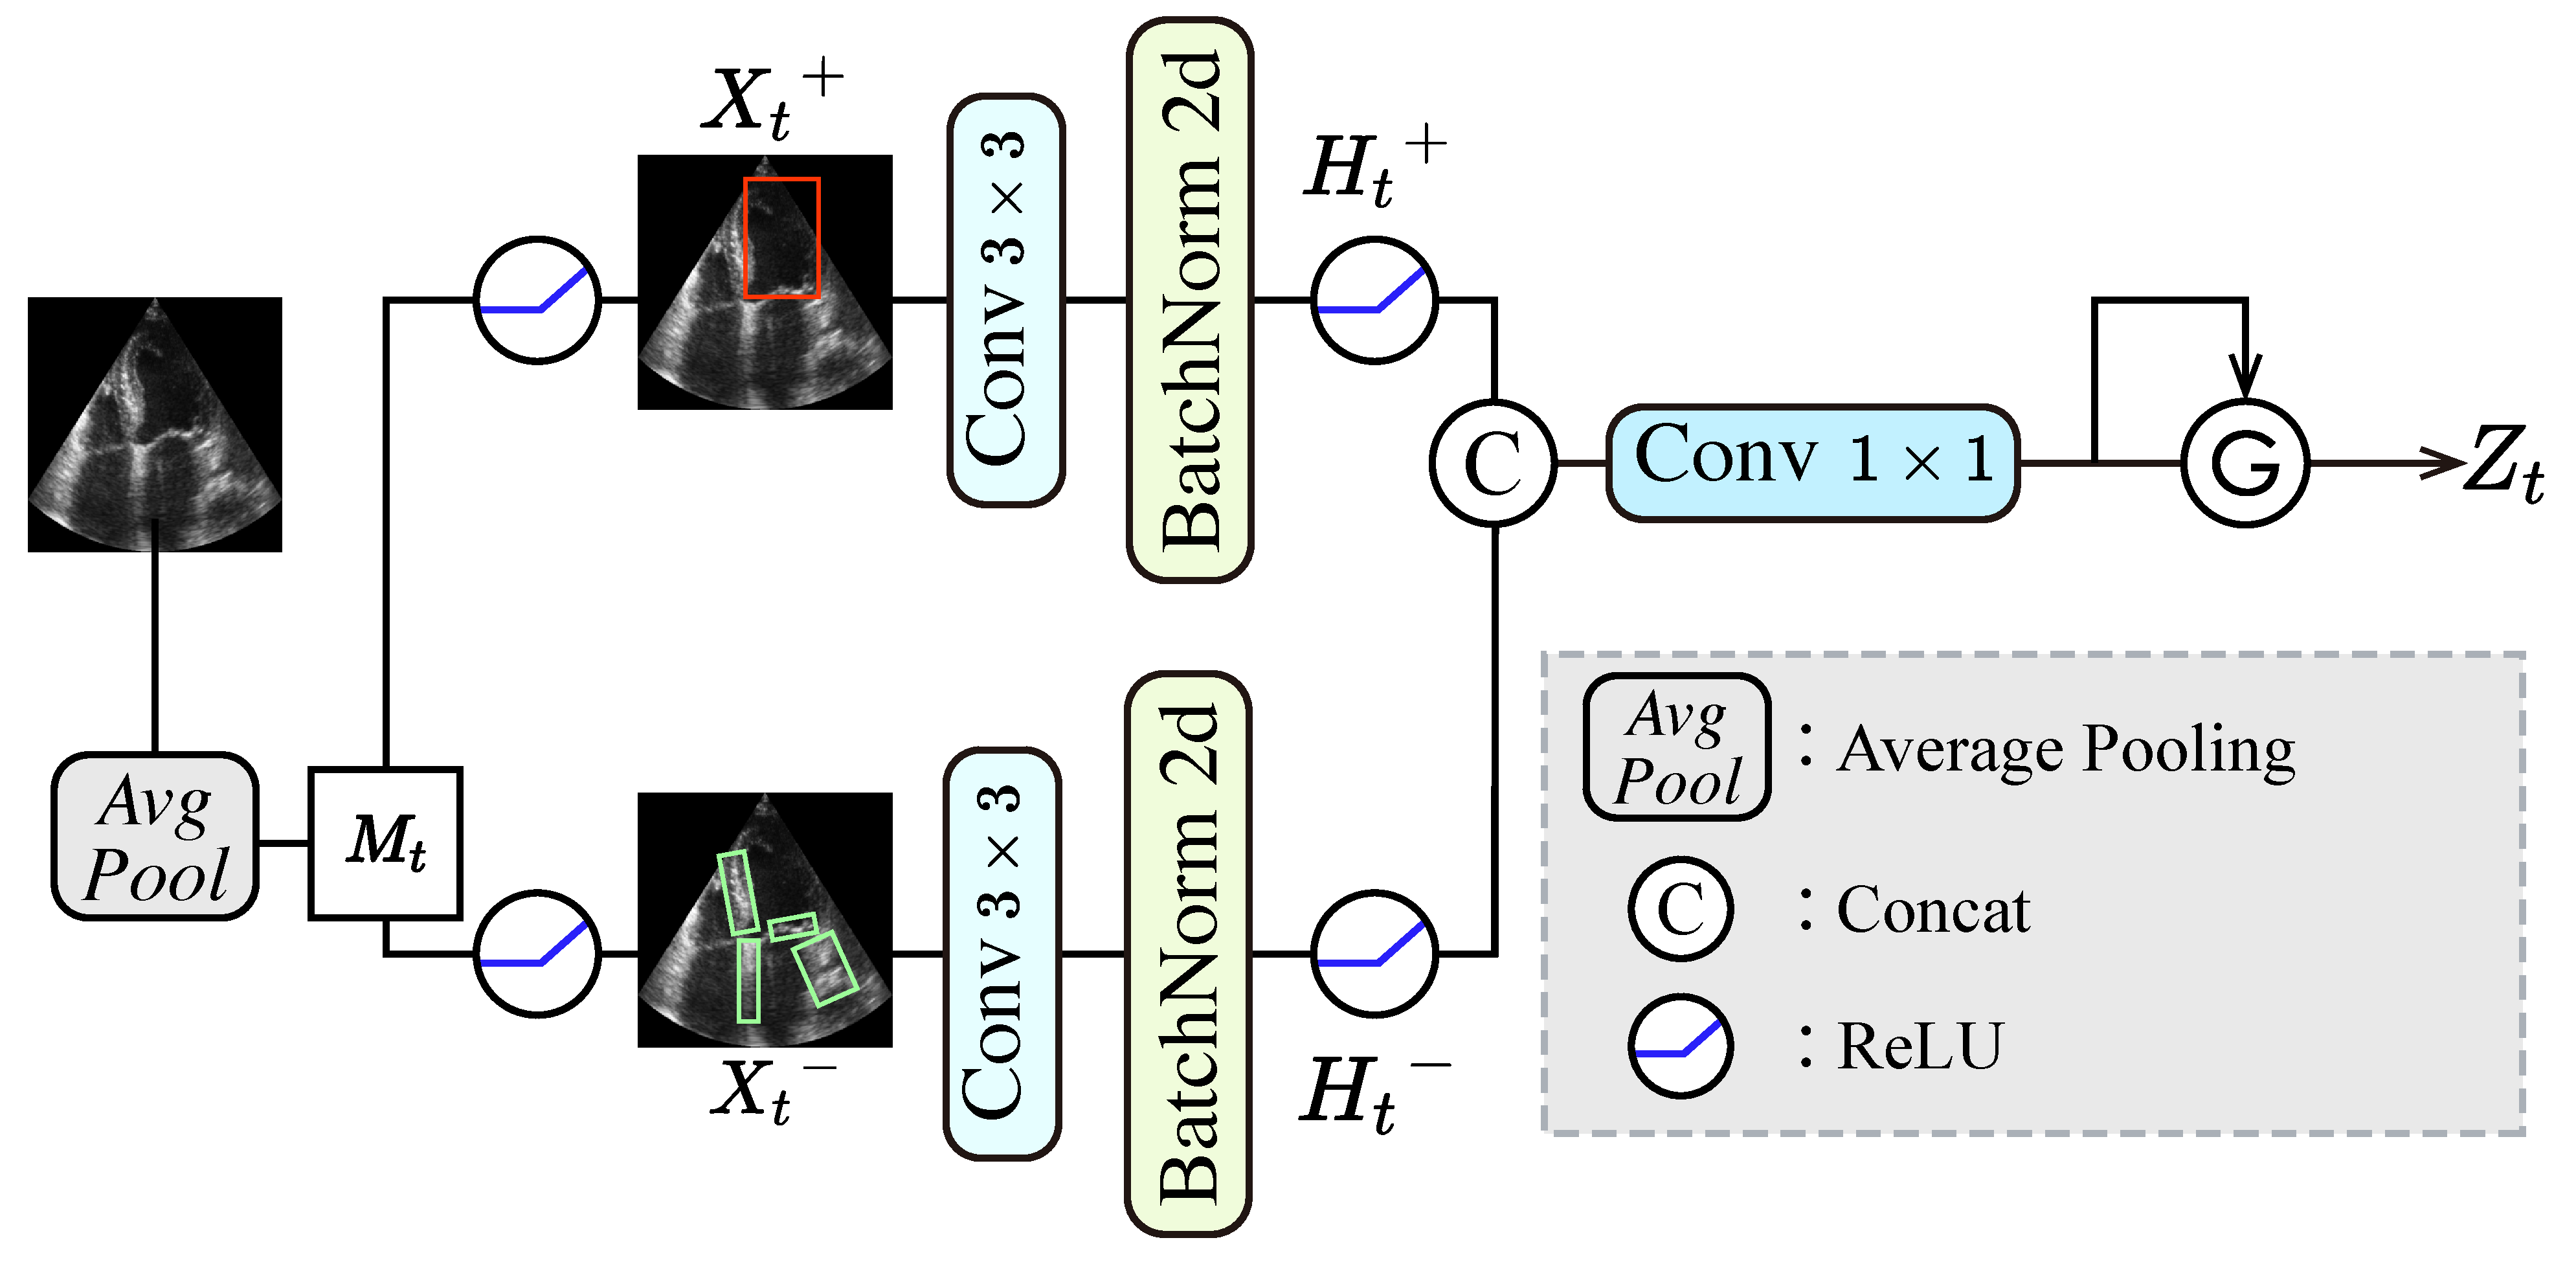
\includegraphics[width=1.0\linewidth]{fig/apfe/fig_apfe.pdf}
    \caption{Illustration of the APFE module.
    APFE decomposes the input into high- and low-intensity components, processes them via dual convolutional branches, and fuses them through a gated mechanism to produce enhanced features $\mathbf{Z}_t$.}
    \label{fig:apfe}
\end{figure}

\noindent
\textbf{Anatomical prior-aware fusion.}
To transform these decoupled components into high-level semantic features, we employ a dual-path strategy:
\begin{equation}
    \mathbf{H}_t^{+} = \phi^{+}(\mathbf{X}_t^{+}), \quad \mathbf{H}_t^{-} = \phi^{-}(\mathbf{X}_t^{-}),
\end{equation}
where $\phi^{+}$ and $\phi^{-}$ are unshared $3\times3$ Conv-BN-ReLU blocks.
This design enables dedicated pathways to separately handle structural geometry via $\phi^{+}$ and region-level semantics via $\phi^{-}$, respectively.
These specialized features are subsequently fused via an adaptive gating mechanism:
\begin{equation}
\label{eq:gating}
\begin{aligned}
    \lambda_t &= \sigma\!\left( \mathbf{W}_g \left[\mathbf{H}_t^{+};\, \mathbf{H}_t^{-}\right] \right), \\
    \mathbf{Z}_t &= \lambda_t \odot \mathbf{H}_t^{+} + (1 - \lambda_t) \odot \mathbf{H}_t^{-},
\end{aligned}
\end{equation}
where $\mathbf{W}_g$ denotes a $1\times1$ convolutional layer, $[\cdot ; \cdot]$ denotes channel-wise concatenation, and $\sigma$ is the sigmoid activation that produces a per-pixel attention map $\alpha_t \in \mathbb{R}^{B\times C\times H\times W}$.
By integrating APFE, the framework generates noise-resilient structural features $\mathbf{Z}_t$ that preserve fine anatomical boundaries decoupled from acoustic artifacts.
These refined features serve as stable key-value inputs for the subsequent sequence modeling process, enabling precise delineation of endocardial contours across varying imaging depths and cardiac phases.